\begin{description}
\item[address space] (of a process) contains all of the memory state of the
running program: the \textbf{code} of the program (the instructions); The running program uses a \textbf{stack} to keep track of where it is in function call chain as well as to allocate local variables and pass parameters and return values to and from routines; the \textbf{heap} is used for dynamically-allocated, user-managed memory, etc.  It is the running program’s view of memory in the system

\item[Access Control List (ACL)]  Access control lists are a more general and powerful way to represent exactly who can access a given resource. In a file system, this enables a user to create a very specific list of who can and cannot read a set of files, in contrast to the somewhat limited owner/group/everyone model of permissions bits.

\item[amortization] The general technique of amortization is commonly used in systems when there is a fixed cost to some operation. By incurring that cost less often (i.e., by performing the operation fewer times), the total cost to the system is reduced. For example, if the time slice is set to 10 ms, and the context-switch cost is 1 ms, roughly 10\% of time is spent context switching and is thus wasted. If we want to \emph{amortize} this cost, we can increase the time slice, e.g., to 100 ms. In this case, less than 1\% of time is spent context switching, and thus the cost of time-slicing has been amortized.

\item[atomicity violation] The desired serializability among multiple memory accesses is violated (i.e. a code region is intended to be atomic, but the atomicity is not enforced during execution)

\item[basepointer-based consistency (BBC, journaling)] (at Wisconsin) In this technique, no ordering is enforced between writes. To achieve consistency, an additional back pointer is added to every block in the system; for example, each data block has a reference to the inode to which it belongs. When accessing a file, the file system can determine if the file is consistent by checking if the forward pointer (e.g., the address in the inode or direct block) points to a block that refers back to it. If so, everything must have safely reached disk and thus the file is consistent; if not, the file is inconsistent, and an error is returned. By adding back pointers to the file system, a new form of lazy crash consistency can be attained

\item[batch process] long-running background tasks: response time not important, cares for long run times (reduce the cost of context switches, cares for lots of CPU, not when)

\item[checkpoint region (CR)] The checkpoint region contains pointers to (i.e., addresses of) the latest pieces of the inode map, and thus the inode map pieces can be found by reading the CR first. The overall structure of the on-disk layout contains a checkpoint region (which points to the latest pieces of the inode map); the inode map pieces each contain addresses of the inodes; the inodes point to files (and directories) just like typical UNIX file systems.

\item[condition variable] an explicit queue that threads can put themselves on when some state of execution (i.e., some \textbf{condition}) is \emph{not} as desired (by \textbf{waiting} on the condition); some other thread, when it changes said state, can then wake one (or more) of those waiting threads and thus allow them to continue (by signaling on the condition). The idea goes back to Dijkstra's use of ``private semaphores''; a similar idea was later named a ``condition variable'' by Hoare in his work on monitors.

\item[consistent-update problem] The problem occurs on a write to any RAID that has to update multiple disks during a single logical operation. In this case, let us assume we are considering a mirrored disk array. Imagine the write is issued to the RAID, and then the RAID decides that
it must be written to two disks, disk 0 and disk 1. The RAID then issues
the write to disk 0, but just before the RAID can issue the request to disk
1, a power loss (or system crash) occurs. In this unfortunate case, let us
assume that the request to disk 0 completed (but clearly the request to
disk 1 did not, as it was never issued).
The result of this untimely power loss is that the two copies of the block
are now \textbf{inconsistent}; the copy on disk 0 is the new version, and the copy
on disk 1 is the old. What we would like to happen is for the state of both
disks to change \textbf{atomically}, i.e., either both should end up as the new
version or neither.
The general way to solve this problem is to use a \textbf{write-ahead log} of some
kind to first record what the RAID is about to do (i.e., update two disks
with a certain piece of data) before doing it. By taking this approach, we
can ensure that in the presence of a crash, the right thing will happen; by
running a \textbf{recovery} procedure that replays all pending transactions to the
RAID, we can ensure that no two mirrored copies (in the RAID-1 case)
are out of sync.
One last note: because logging to disk on every write is prohibitively
expensive, most RAID hardware includes a small amount of non-volatile
RAM (e.g., battery-backed) where it performs this type of logging. Thus,
consistent update is provided without the high cost of logging to disk.

\item[context switch] is a mechanism that allows the OS to store the current process state and switch to some other, previously stored context.

\item[convey effect] a number of relatively-short potential consumers of a resource get queued behind a heavyweight resource consumer

\item[Copy-on-write (COW)] This technique never overwrites files or directories in place; rather, it places new updates to previously unused locations on disk. After a number of updates are completed, COW file systems flip the root structure of the file system to include pointers to the newly updated structures. Doing so makes keeping the file system consistent straightforward.  LFS introduces a new approach to updating the disk. Instead of overwriting files in places, LFS always writes to an unused portion of the disk, and then later reclaims that old space through cleaning. This approach, which in database systems is called \textbf{shadow paging} and in file-system-speak is sometimes called copy-on-write, enables highly efficient writing, as LFS can gather all updates into an in-memory segment and then write them out together sequentially

\item[crash-consistency problem] One major challenge faced by a file system is how to update persistent data structures despite the presence of a \textbf{power loss} or \textbf{system crash}. Specifically, what happens if, right in the middle of updating on-disk structures, someone trips over the power cord and the machine loses power? Or the operating system encounters a bug and crashes? What we’d like to do ideally is move the file system from one consistent state (e.g., before the file got appended to) to another atomically (e.g., after the inode, bitmap, and new data block have been written to disk). Because of power losses and crashes, updating a persistent data structure can be quite tricky, and leads to a new and interesting problem in file system implementation, known as the crash-consistency (consistent-update) problem.

\item[Deadlock Avoidance] Avoidance requires some global knowledge of which locks various threads might grab during their execution, and subsequently \textbf{schedules} said threads in a way as to guarantee no deadlock can occur.

\item[Directory] a collection of tuples, each of which contains a human-readable name and low-level name to which it maps. Each entry refers either to another directory or to a file. Each directory also has a low-level name (i-number) itself. A directory always has two special entries: the \textbf{\texttt{.}} entry, which refers to itself, and the \textbf{\texttt{..}} entry, which refers to its parent.

\item[Directory Tree/Hierarchy] organizes all files and directories into a large tree, starting at the \textbf{root} (often represented as \texttt{/}).

\item[dynamic partitioning] The dynamic approach is more flexible, giving out differing amounts of the resource over time; for example, one user may get a higher percentage of disk bandwidth for a period of time, but then later, the system may switch and decide to give a different user a larger fraction of available disk bandwidth.

\item[DMI]  Intel’s proprietary DMI (Direct Media Interface), for connecting I/O Chip

\item[eSATA] external SATA represent an evolution of storage interfaces over the past decades, with each step forward increasing performance to keep pace with modern storage devices

\item[fail-stop fault model (disk)]  In this model, a disk can be in exactly one of two states: working or failed. With a working disk, all blocks can be read or written. In contrast, when a disk has failed, we assume it is permanently lost. One critical aspect of the fail-stop model is what it assumes about fault detection. Specifically, when a disk has failed, we assume that this is easily detected.

\item[File] A file is an array of bytes which can be created, read, written, and deleted. It has a low-level name (i.e., a number) that refers to it uniquely. The low-level name is often called an \textbf{inode number} (\textbf{i-number}).  A file, as presented to the user via a file name, is essentially a “pointer” to the underlying inode that structure in the disk that contains the actual data. Different ways to refer to a file:
\begin{enumerate*}[label={\alph*.},font={\color{red!50!black}\bfseries}]
\item file name (human readable)
\item inode number (persistent ID)
\item file descriptor (process view)
\end{enumerate*}

\item[File Descriptor] To access a file, a process must use a system call (usually, \texttt{open()}) to request permission from the operating system. If permission is granted, the OS returns a \textbf{file descriptor} (an \texttt{int}, private per process and is used in UNIX systems), which can then be used for read or write access, as permissions and intent allow.  Thus, a file descriptor is a capability, i.e., an opaque handle that gives you the power to perform certain operations.  When you first open another file, it will almost certainly be file descriptor \textbf{3}, because In Linux, by default a process already has \textbf{3} file descriptors:
\begin{enumerate*}[label={\alph*.},font={\color{red!50!black}\bfseries}]
\item standard input (0)
\item standard output (1)
\item standard error (2)
\end{enumerate*}


\item[File Type]  In some systems (Windows), a file's name carry a structure: a two-part name, separated by a \texttt{.}: \texttt{filename.ext}. This is mostly a \textbf{convention}, so no enforcement on the data contained in the file. Other systems adopt an untyped view: no convention to relate to specific content of the file.

\item[free list] In early file systems, a single pointer in the super block was kept to point to the first free block; inside that block the next free pointer was kept, thus forming a list through the free blocks of the system. When a block was needed, the head block was used and the list updated accordingly.

\item[garbage collection (file system)] In LFS, it repeatedly writes the latest version of a file (including its inode and data) to new locations on disk. This process, while keeping writes efficient, implies that LFS leaves old versions of file structures scattered throughout the disk. We (rather unceremoniously) call these old versions garbage.

\item[Hill's law] One early source is Mark Hill's dissertation, which studied how to design caches for CPUs. Hill found that simple direct-mapped caches worked better than fancy set-associative designs (one reason is that in caching, simpler designs enable faster lookups). As Hill succinctly summarized his work: ``Big and dumb is better.'' And thus we call this similar advice Hill's Law.

\item[idle process] If all processes are blocked, \mb{idle} procs should be scheduled. Modern kernels use a low priority idle process that is scheduled and executes if no other process iss ready. The idle process never blocks or executes any I/O. Without the idle process, the scheduler would have to check if no processes are ready to run and would have to conservatively take action. The idle process guarantees that there is always at least one process to run.

\item[inode] Index node. The inode is the generic name that is used in many file systems to describe the structure that holds the metadata for a given file, such as its length, permissions, and the location of its constituent blocks. The name
goes back at least as far as UNIX (and probably further back to Multics if not earlier systems); it is short for index node, as the inode number is used to index into an array of on-disk inodes in order to find the inode of that number. The design of the inode is one key part of file system design. Most modern systems have some kind of structure like this for every file they track, but perhaps call them different things (such as dnodes, fnodes, etc.).

\item[immediate reporting (fs journaling)] With write buffering enabled (sometimes called immediate reporting), a disk will inform the OS the write is complete when it simply has been placed in the disk’s memory cache, and has not yet reached disk

\item[interactive process] low latency foreground tasks: response time critical, short bursts (context switching cost not important, not much CPU needed but frequently)

\item[Lauer's law] As Hugh Lauer said, when discussing the construction of the Pilot operating system: ``If the same people had twice as much time, they could produce as good of a system in half the code.''

\item[limited direct execution] let the program run directly on the hardware; however, at certain key points in time (such as when a process issues a system call, or a timer interrupt occurs), arrange so that the OS gets involved and makes sure the ``right'' thing happens.   Thus, the OS, with a little hardware support, tries best to get out of the way of the running program, to deliver an \emph{efficient} virtualization.

\item[lock] Generally, Programmers annotate source code with locks, putting them around critical sections, and thus ensure that any such critical section executes as if it were a single \textbf{atomic} instruction.

\item[Log-structured File System] introduced by Rosenblum and Ousterhout, When writing to disk, LFS first buffers all updates (including metadata!) in an in-memory \textbf{segment} (large-ish chunk LFS uses to group writes); when the segment is full, it is written to disk in one long, sequential transfer to an unused part of the disk. LFS never overwrites existing data, but rather \emph{always} writes segments to free locations. Because segments are large, the disk (or RAID) is used efficiently, and performance of the file system approaches its zenith.

\item[LRU] least recently used: take advantage of locality in the memory-reference stream, assuming it is likely that an entry that has not recently been used is a good
candidate for eviction.

\item[mesa semantics] Signaling a thread only wakes them up; it is thus a hint that the state of the world has changed (in this case, that a value has been placed in the buffer), but there is no guarantee that when the woken thread runs, the state will still be as desired. This interpretation of what a signal means is often referred to as Mesa semantics (1st implemented in Mesa programming language). In contrast, \textbf{Hoare semantics} requires the woken thread be run immediately.  Most (if not all) systems use the Mesa semantics.

\item[memory virtualization] OS maps user program address space to physical memory address.

\item[memory management unit] the part of the processor that helps with address translation (base and bounds registers kept on the chip).

\item[most-recently-used (MRU)] MostFrequently-Used (MFU) and Most-Recently-Used (MRU). In most cases (not all!), these policies do not work well, as they ignore the locality most programs exhibit instead of embracing it.

\item[mutex] The name that the POSIX library uses for a lock, as it is used to provide mutual exclusion between threads, i.e., if one thread is in the critical section, it excludes the others from entering until it has completed the section.

\item[Open File Table] Each file descriptor is a private, per-process entity. Each process maintains an array of file descriptors, each of which refers to an entry in the system-wide \textbf{open file table}. The entry therein tracks which file this access refers to, the \textbf{current offset} of the file (i.e., which part of the file the next read or write will access), and other relevant details such as whether the file is readable or writable

\item[order violation] The desired order between two (groups of) memory accesses is flipped (i.e., A should always be executed before B, but the order is not enforced during execution)

\item[ordered journaling] User data must be written to disk before metadata and bitmap updates, otherwise when file systems recovers, since the inode points to old value (garbage), garbage will be copied and replayed to data block. Windows NTFS and SGI’s XFS both use some form of metadata journaling. Linux ext3 gives you \textbf{3} options (journaling modes)
  \begin{enumerate*}[label={\alph*.},font={\color{red!50!black}\bfseries}]
  \item data: logs both metadata and ata in journal
  \item ordered: logs metadata only, and data write must happen before journal metadata write/commit
  \item writeback (unordered): same as ordered but data write can happen at any time.
  \end{enumerate*}
All of these modes keep metadata consistent; they vary in their semantics for data.

\item[optimistic crash consistency] technique to reduce the number of times a journal protocol has to wait for disk writes to complete.  this new approach issues as many writes to disk as possible by using a generalized form of the transaction checksum, and includes a few other techniques to detect inconsistencies should they arise. For some workloads, these optimistic techniques can improve performance by an order of magnitude. However, to truly function well, a slightly different disk interface is required

\item[paging] Chop memory into \emph{fixed-sized} pieces, each called a \textbf{page} (usually 4KB)

\item[page frame] physical memory viewed as an array of fixed-sized slots called page frames; each of these frames can contain a single virtual-memory page.

\item[page table] s a per-process data structure maintained by OS.  Its major role is to store address translations for each of the virtual pages of the address space, thus letting us know where in physical memory each page resides.

\item[page fault] the act of accessing a page that is not in physical memory.  Upon a page fault, the OS is invoked to service the page fault.  Virtually all systems handle page faults in software.

\item[pre-allocation policy] When allocating data blocks for a new file. For example, some Linux file systems, such as ext2 and ext3, will look for a sequence of blocks (say 8) that are free when a new file is created and needs data blocks; by finding such a sequence of free blocks, and then allocating them to the newly-created file, the file system guarantees that a portion of the file will be contiguous on the disk, thus improving performance. Such a \textbf{pre-allocation} policy is thus a commonly-used heuristic when allocating space for data blocks.

\item[preemptive scheduling] Virtually all modern schedulers are preemptive, and quite willing to stop one process from running in order to run another. This implies that the scheduler employs the mechanisms we learned about previously; in particular, the scheduler can perform a \textbf{context switch}, stopping one running process temporarily and resuming (or starting) another. In the old days of batch computing, a number of \textbf{non-preemptive} schedulers were developed; such systems would run each job to completion before considering whether to run a new job.

\item[process] At any point in time, the process can be described by its state: the contents of memory in its \textbf{address space}, the contents of CPU registers (including the \textbf{program counter} and \textbf{stack pointer}, among others), and information about I/O (such as open files which can be read or written). The \textbf{process API} consists of calls programs can make related to processes. Typically, this includes creation (\texttt{fork()}), destruction (\texttt{exit(), kill(), wait()}), and other useful calls. A process can launch multiple \textbf{threads} of execution in the same address space. Each thread receives its own stack but they share global data, code, and heap.

\item[process states] Processes exist in one of many different process states, including \mb{running} (\texttt{RUNNING}), \mb{ready to run} \texttt{RUNNABLE}, and blocked (\texttt{SLEEPING}), \mb{new}: process being created (to ensure it will not be scheduled), \mb{dead}: this process has terminated (whether parent process has not read out the return value yet). Different events (e.g., getting scheduled or descheduled, or waiting for an I/O to complete) transition a process from one of these states to the other.

\item[process control block (PCB)] A \textbf{process list} (aka. \textbf{task list}) contains information about all processes in the system. Each entry is found in what is sometimes called a process control block (PCB, aka \textbf{process descriptor}) , which is really just a structure that contains information about a specific process.

\item[proportional-share scheduler] (aka fair-share scheduler) Proportional-share is based around a simple concept: instead of optimizing for turnaround or response time, a scheduler might instead try to guarantee that each job obtain a certain percentage of CPU time. For example, lottery scheduling.

\item[recursive update problem]  The problem arises in any file system that never updates in place (such as LFS), but rather moves updates to new locations on the disk. Specifically, whenever an inode is updated, its location on disk changes. If we hadn’t been careful, this would have also entailed an update to
the directory that points to this file, which then would have mandated
a change to the parent of that directory, and so on, all the way up the file
system tree. LFS cleverly avoids this problem with the inode map. Even though
the location of an inode may change, the change is never reflected in the
directory itself; rather, the imap structure is updated while the directory
holds the same name-to-inode-number mapping. Thus, through indirection, LFS avoids the recursive update problem.

\item[Redundant Array of Inexpensive Disks (RAIDs)] , a technique to use multiple disks in concert to build a faster, bigger, and more reliable disk system. The term was introduced in the late 1980s by a group of researchers at U.C. Berkeley (led by Professors David Patterson and Randy Katz and then student Garth Gibson); Externally, a RAID looks like a disk: a group of blocks one can read or write. A RAID system is often built as a separate hardware box, with a standard connection (e.g., SCSI, or SATA) to a host. Internally, the RAID is a complex beast, consisting of multiple disks, memory (both volatile and non-), and one or more processors to manage the system. A hardware RAID is very much like a computer system, specialized for the task of managing a group of disks.

\item[Round-Robin (RR) scheduling] The basic idea is simple: instead of running jobs to completion, RR runs a job for a \textbf{time slice} (sometimes called a scheduling quantum) and then switches to the next job in the run queue. It repeatedly does so until the jobs are finished. \mr{good for response time, worst for turnaround time}

\item[SATA] Serial ATA (AT Attachment)

\item[scheduling policy] A scheduling policy determines \textbf{which} process should run next. If there is only one “ready” process then the answer is easy. If there are more processes then the policy decides in which order processes
execute. The context switch mechanism takes care of \textbf{how} the kernel switches from one process to another, namely by storing its context and restoring the context of the other process.

\item[segmentation] Chop memory into \textsw{variable-sized} chunks and allocate them based on needs (e.g in base/bound or segmentation approaches)

\item[segmentation fault] a violation or error arising from a memory access on a segmented machine to an illegal address.

\item[Shorted Time First (SFJ)]  scheduling policy that runs the shortest job first, then the next shortest, and so on.

\item[Shorted Time-to-Completion First (STCF)] aka. Preemptive Shortest Job First (PSJF) scheduler: Any time a new job enters the system, the STCF scheduler determines which of the remaining jobs (including the new job) has the least time left, and schedules that one. \mr{great for turnaround time, but not good for response time}: If three jobs arrive at the same time, for example, the third job has to wait for the previous two jobs to run in their entirety before being scheduled just once.

\item[small-write problem] both RAID-4 and RAID-5 have the small-write problem where a logical write to a single block causes 4 physical I/Os to take place.

\item[soft updates (journaling)] introduced by Ganger and Patt. This approach carefully orders all writes to the file system to ensure that the on-disk structures are never left in an inconsistent state. For example, by writing a pointed-to data block to disk \emph{before} the inode that points to it, we can ensure that the inode never points to garbage; similar rules can be derived for all the structures of the file system. Implementing Soft Updates can be a challenge, however, requiring
intricate knowledge of each file system data structure and thus adds a fair amount of complexity to the system.

\item[sparse address space] large address spaces with large amounts of unused address space

\item[static partitioning] When dividing a resource among different clients/users, you can use either static partitioning or dynamic partitioning (see above). The static approach simply divides the resource into fixed proportions once; for example, if there're 2 possible users of memory, can give some fixed fraction of memory to one user and the rest to the other.

\item[starvation (scheduling)]  if there are ``too many'' interactive jobs in the system, they will combine to consume all CPU time, and thus long-running jobs will never receive any CPU time (they \textbf{starve}). We'd like to make some progress on these jobs even in this scenario


\item[ticket currency (lottery scheduling)] Currency allows a user with a set of tickets to allocate tickets among their own jobs in whatever currency they
would like; the system then automatically converts said currency into the
correct global value. For example, assume users A and B have each been given 100 tickets. User A is running two jobs, A1 and A2, and gives them each 500 tickets (out of 1000 total) in A's currency. User B is running only 1 job and gives it 10 tickets (out of 10 total). The system converts A1's and A2's allocation from 500 each in A's currency to 50 each in the global currency; similarly, B1's 10 tickets is converted to 100 tickets. The lottery is then held over the global ticket currency (200 total) to determine which job runs.
\begin{lstlisting}[language=bash]
User A -> 500 (A's currency) to A1 -> 50 (global currency)
       -> 500 (A's currency) to A2 -> 50 (global currency)
User B -> 10  (B's currency) to B1  -> 100 (global currency)
\end{lstlisting}

\item[ticket inflation] With inflation, a process can temporarily raise or lower the number of tickets it owns. Of course, in a competitive scenario with processes that do not trust one another, this makes little sense; one greedy process could give itself a vast number of tickets and take over the machine. Rather, inflation can be applied in an environment where a group of processes trust one another; in such a case, if any one process knows it needs more CPU time, it can boost its ticket value as a way to reflect that need to the system, all without communicating with any other processes.

\item[ticket transfer] With transfers, a process can temporarily hand off its tickets to another process. This ability is especially useful in a client/server setting, where a client process sends a message to a server asking it to do some work on the client’s behalf. To speed up the work, the client can pass the tickets to the server and thus try to maximize the performance of the server while the server is handling the client’s request. When finished, the server then transfers the tickets back to the client and all is as before.

\item[time-space-trade-offs] Usually, if you wish to make access to a particular data structure faster, you will have to pay a space-usage penalty for the structure.

\item[throttling] an approach where programmer decides upon a threshold for ``too many'', and then use a semaphore to limit the number of threads concurrently executing the piece of code in question.  This is also a form of \textbf{admission control}. Imagine that you create hundreds of threads to work on some problem in parallel. However, in a certain part of the code, each thread acquires a large amount of memory to perform part of the computation; let’s call this part of the code the \emph{memory-intensive region}. If \emph{all} of the threads enter the memory-intensive region at the same time, the sum of all the memory allocation requests will exceed the amount of physical memory on the machine. As a result, the machine will start thrashing (i.e., swapping pages to and from the disk), and the entire computation will slow to a crawl.  A simple semaphore can solve this problem. By initializing the value of the semaphore to the maximum number of threads you wish to enter the memory-intensive region at once, and then putting a \texttt{sem\_wait()} and \texttt{sem\_post()} around the region, a semaphore can naturally throttle the number of threads that are ever concurrently in the dangerous region of the code.

\item[time sharing] Time sharing is a basic technique used by an OS to share a resource. By allowing the resource to be used for a little while by one entity, and then a little while by another, and so forth, the resource in question (e.g., the CPU, or a network link) can be shared by many. The counterpart of time sharing is \textbf{space sharing}, where a resource is divided (in space) among those who wish to use it. For example, disk space is naturally a space-shared resource; once a block is assigned to a file, it is normally not assigned to another file until the user deletes the original file.

\item[Time of Check To Time of Use (TOCTTOU)] McPhee notes that ``... if there exists a time interval between a validity-check and the operation connected with that validity-check, [and,] through multitasking, the validity-check variables can deliberately be changed during this time interval, resulting in an invalid operation being performed by the control program'', thus this problem.  There are not any simple and great solutions to the TOCTTOU problem. One approach is to reduce the number of services that need root privileges to run, which helps. The \texttt{O\_NOFOLLOW} flag makes it so that \texttt{open()} will fail if the target is a symbolic link, thus avoiding attacks that require said links.

\item[translation-lookaside buffer (TLB)] part of the chip’s memory-management unit (MMU), and is simply a hardware cache of popular virtual-to-physical address translations; thus, a better name would be an address-translation cache.

\item[track buffer] modern disks are much smarter: they internally read the entire track in and buffer it in an internal disk cache (often called a track buffer for this very reason). Then, on subsequent reads to the track, the disk will just return the desired data from its cache. File systems thus no longer have to worry about these incredibly low-level details.


\item[unwritten contract of disk drives] Specifically, one can usually assume that accessing two blocks near one-another within the drive’s address space will be faster than accessing two blocks that are far apart. One can also usually assume that accessing blocks in a contiguous chunk (i.e., a sequential read or write) is the fastest access mode, and usually much faster than any more random access pattern.

\item[virtual address] All that in user program address space

\item[zombie process] A process is in a zombie state if it’s terminated but not yet removed from the process table. This could happen if the parent process did not execute a \texttt{wait()} syscall for a child process, and the child process terminates. Always execute \texttt{wait()} syscall to prevent child procs from becoming zombies. Alternatively, handle the \texttt{SIGCHILD} signal, triggered when a child process terminates.  Unix/Linux distinguishes two states of a terminated process: a \texttt{zombie} state and a \texttt{dead} state.
\end{description}


%%%%%%%%%%%%%%%%%%%%%%%%%%%% PROCESS STUFF %%%%%%%%%%%%%%%%%%%%%%%%%%%%
\section*{Process API (available on any modern OS)}
The process API enables a proc to control itself and other procs through a set of system calls:
  \begin{enumerate*}[label={\alph*.},font={\color{red!50!black}\bfseries}]
  \item \texttt{fork()} creates a new child process (a copy of the process)
  \item \texttt{exec()} executes a new program
  \item \texttt{exit()} terminates the current process
  \item \texttt{wait()} blocks parent until child terminates
  \end{enumerate*}
\begin{itemize}
\item Create: An operating system must include some method to create new processes. When you type a command into the shell, or double-click on an application icon, the OS is invoked to create a new process to run the program you have indicated
\item Destroy: As there is an interface for process creation, systems also provide an interface to destroy processes forcefully. Of course, many processes will run and just exit by themselves when complete; when they don’t, however, the user may wish to kill them, and thus an interface to halt a runaway process is quite useful
\item Wait: it is useful to wait for a process to stop running; thus some kind of waiting interface is often provided
\item Miscellaneous Control: Other than killing or waiting for a process, there are sometimes other controls that are possible. For example, most operating systems provide some kind of method to suspend a process (stop it from running for a while) and then resume it (continue)
\item Status: there're usually interfaces to get some status info about a process as well how long it has run for or what state it is in
\end{itemize}
\section*{API \texttt{fokr()} (return twice)}
\begin{enumerate}
\item OS allocates data structures for new process (child)
\item OS makes a copy of caller's (parent's) address space
\item the child is made ready and added to the list of processes
\item \texttt{fork()} returns different values for parent(child pid)/child(0)
\item parent and child continue execution in \mo{their own separate copy} of their address space
\end{enumerate}
\section*{API \texttt{exec()} (never returns on success; returns -1 on error/failure)}
\begin{itemize}
\item replaces address space, load new program from disk
\item program can pass cmd line args and environment variables
\item old address space/state destroyed except for \texttt{STDIN}, \texttt{STDOUT}, \texttt{STDERR}, allowing parent to redirect/rewire child's output
\end{itemize}
\section*{API \texttt{wait()} (wait for child to reap it) }
\begin{itemize}
\item child processes tied to their parent(s)
\item \texttt{exit(int retval)} takes a return value argument
\item parent can \texttt{wait()} for termination of child and read child's return val
\end{itemize}
\section*{Reasons for the need for \texttt{fork()} and \texttt{exec()}}
Assume a user wants to start a different program. For that, the operating system needs to create a new process and create a new address space to load the program:
\begin{itemize}
\item \texttt{fork()} creates a new process with a copy of this address space
\item \texttt{exec()} creates a new address space for a program
\item \texttt{clone()} adds a thread (of execution) to this address space
\end{itemize}
\section*{\texttt{init} process (\texttt{pid == 1}, parent of all) and orphan process}
\begin{itemize}
\item \texttt{init} responsible for starting other processes, reaping `zombie's, adopting orphans
\item when parent terminates but one of its children still running $\to$ orphan
\item orphans processes adopted by \texttt{init} process in the end
\item needed particularly for background (long-running daemon) services:
  \begin{enumerate*}[label={\alph*.},font={\color{red!50!black}\bfseries}]
  \item parent process deliberately creates a child
  \item parent exits and orphans the child
  \item \texttt{init} adopts the child (say, \texttt{systemd})
  \item common examples: web/databse servers, monitoring programs
  \end{enumerate*}
\item benefits:
  \begin{enumerate*}[label={\alph*.},font={\color{red!50!black}\bfseries}]
  \item runs independently
  \item continues running even if user logs out
  \item clean process hierarchy
  \item no direct parent needed to monitor it
  \end{enumerate*}
\end{itemize}
\section*{Process States (simplified 3 states)}
\begin{enumerate}
\item Running: In the running state, a process is running on a processor. This means it is executing instructions
\item Ready: In the ready state, a process is ready to run but for some reason the OS has chosen not to run it at this given moment.
\item Blocked: In the blocked state, a process has performed some kind of operation that makes it not ready to run until some other event takes place. For example: when a process initiates an I/O request to a disk, it becomes blocked and thus some other process can use the processor
\end{enumerate}
\section*{Distinction program / process / thread}
\begin{itemize}
\item program: consists of an executable on disk. contains all information to boostrap a process
\item a running instance of a program; has data section and stack initialized
\item a process can have multiple threads in the same address space (computing on the same data)
\end{itemize}
\section*{Issues with running program directly on hardware}
\begin{itemize}
\item Process could do something illegal (read/write to memory that does not belong to the process, access hardware directly)
\item Process could run forever (OS must stay in control)
\item Process could do something slow, e.g., I/O (OS may want to switch to another process)
\end{itemize}
\textbf{Solution}: OS maintains some control with help from hardware. For example, the OS maintains timers to intercept the execution at regular intervals and the process may not execute privileged instructions that access the hardware directly.
\section*{Process isolation policy}
\begin{itemize}
\item most operation systems isolate processes from
  \begin{enumerate*}[label={\alph*.},font={\color{red!50!black}\bfseries}]
  \item each other
  \item the OS
  \end{enumerate*}
\item isolation is a core requirement for security:
  \begin{enumerate*}[label={\alph*.},font={\color{red!50!black}\bfseries}]
  \item constrains bugs to the process
  \item enables privilege isolation
  \item enables compartmentalization (breaking complex systems into independent fault domains)
  \end{enumerate*}
\end{itemize}
\section*{Process isolation mechanism}
\begin{itemize}
\item Virtual memory: one (virtual) address space per process
\item Different execution modes: OS executes at super privileges; procs at user mode
\end{itemize}
\section*{Kernel switch from one process to another (transparent to process)}
\begin{itemize}
\item assume one CPU and system has several \texttt{ready} processes
\item processes may \texttt{yeild()} or execute I/O operations
\item OS uses config. timer interrupts to take control back from user procs
\item context switch saves running process's state in kernel data structure
\item context switch restores state of the next-to-run process
\item context switch transfers control to next process and returns
\end{itemize}
\section*{Reasons for context swith}
\begin{itemize}
\item the process completes and/or exits
\item the process executes a slow hardware operation (loading from disk) and OS switches to another ready-to-run task
\item the hardware requires OS help and issue an interrupt
\item the OS decides to preempt the task and switch to another task (i.e. the procs has used up its time slices)
\end{itemize}
\section*{Context switch code and 2 types of saves/restores}
A function call that returns asynchronously: process A starts the execution of the context switch but process B continues execution after the return of the function:
\begin{enumerate*}[label={\alph*.},font={\color{red!50!black}\bfseries}]
\item The function saves all registers in a scratch area (on the process's kernel stack or in a predefined area of the \textsw{task} struct)
\item OS switches address space
\item function restores all registers from the scratch area
\item OS returns to process B
\end{enumerate*}
\begin{enumerate}
\item when timer interrupt occurs: the \mo{user registers} of the running proc get implicitly saved by the \emph{hardware}, using kernel stack of that proc
\item when OS decides to switch from A to B: the \mo{kernel registers} are explicitly saved by the software (i.e., the OS), but this time into memory in the proc structure of the proc
\end{enumerate}
\begin{lstlisting}[language={[x86masm]Assembler}]
# void ctx_swtch(struct context *old, struct context *new)
# Save old registers
movl 4(%esp), %eax # load ptr to old into eax
popl 0(%eax)
 # store old IP to old
movl %esp, 4(%eax) # store stack pointer
movl %ebx, 8(%eax) # store other registers
...
movl %ebp, 28(%eax)
# Load new registers
movl 4(%esp), %eax # load ptr to new into eax
movl 28(%eax), %ebp # restore other registers
...
movl 8(%eax), %ebx
movl 4(%eax), %esp # stack switch (from now on new stack)
pushl 0(%eax)
 # store return addr
ret
 # finally return into new ctxt
\end{lstlisting}
\section*{Why reboot is useful}
\begin{itemize}
\item it moves software back to a known and likely more tested state
\item it also reclaim stale or leaked resources (e.g., memory) which may otherwise be hard to handle
\item reboots are easy to automate
\end{itemize}
\section*{Scheduler metrics and possible goals of a scheduler}
\begin{itemize}
\item \textbf{utilization}: time of CPU executing a program (maximize)
\item \textbf{turnaround time}:  total global time from proc creation to proc exit (minimize)
\item \textbf{response time}: time from ready to being scheduled (minimize)
\item \textbf{fairness}: all procs get same amt of CPU over time (no starvation)
\item \textbf{progress}: allow proc to make forward progress (minimize kernel interrupts)
\end{itemize}
\section*{Key CPU virtualization terms (mechanisms)}
\begin{itemize}
\item Typical user applications run in \mo{user mode}, and use a \mo{system call} to \mo{trap} into the kernel to request operating system services
\item The trap ix saves register state carefully, changes the hardware status to kernel mode, and jumps into the OS to a pre-specified destination: the \mo{trap table}, which must be set up by the OS at boot time, and make sure that they cannot be readily modified by user programs. All of this is part of the \mo{limited direct execution} protocol which runs programs efficiently but without loss of OS control
\end{itemize}
\section*{Stride Scheduling}
a deterministic fair-share scheduler, Each job in the system has a stride, which is inverse in proportion to the number of tickets it has. Given jobs A, B, C with 100, 50, 250 tickets, respectively, we can compute the stride of each by dividing some large number by the number of tickets each process has been assigned. For example, if we divide 10,000 by each of those ticket values, we obtain the following stride values for A, B, and C: 100, 200, and 40. We call this value the \textbf{stride} of each process; every time a process runs, we will increment a counter for it (called its \textbf{pass} value) by its stride to track its global progress.

The scheduler then uses the stride and pass to determine which process should run next. The basic idea is simple: at any given time, pick the process to run that has the \mo{lowest} pass value so far; when you run a process, increment its pass counter by its stride:
\begin{lstlisting}[language=c]
curr = remove_min(queue);      // pick client with min pass
schedule(curr);                // run for quantum
curr->pass += curr->stride;  // update pass using stride
insert(queue, curr);           // return curr to queue
\end{lstlisting}
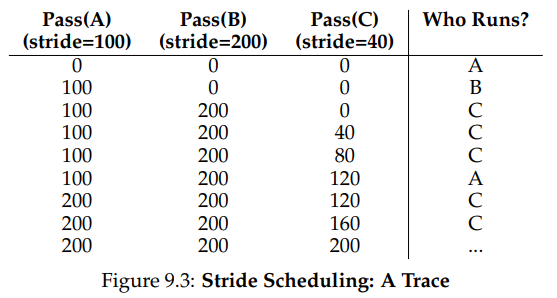
\includegraphics[width=\linewidth]{imgs/sched_stride}
\begin{itemize}
\item 3 processes: A, B, C; stride value: $A = 100\;B = 200\; C=40$
\item $A$ runs 1st (choose arbitrarily) $\to$ \texttt{pass} updated to 100
\item $A$ runs 2nd  $\to$  \texttt{pass} updated to 200
\item $C$ runs 3rd  $\to$  \texttt{pass} updated to 40
\item $C$ runs again (lowest pass)  $\to$  \texttt{pass} updated to 80
\item $C$ runs again (still lowest pass) $\to$ \texttt{pass} updated to 120
\item $A$ runs (next lowest) $\to$  \texttt{pass} updated to 200
\item $C$ runs twice more $\to$ \texttt{pass} updated to 160, then 200
\item all pass values equal 200, above pattern repeat until all jobs done
\item lottery scheduling achieves the proportions probabilistically over time
\item stride sched gets them exactly right at the end of each scheduling cycle
\item lottery has no global state $\to$ much easier to incorporate new procs
\end{itemize}
\section*{RAID Advantages (looks like a big disk to host system)}
\begin{enumerate}
\item performance: multiple disks in parallel can greatly speed up I/O times
\item capacity: large data sets demand large disks
\item reliability: spreading data across multiple disks (without RAID techniques) makes the data vulnerable to the loss of a single disk; with some form of \textbf{redundancy}, RAIDs can tolerate the loss of a disk and keep operating as if nothing were wrong.
\end{enumerate}
\section*{Evaluating RAID: three axes}
\begin{enumerate}
\item capacity: given a set of $N$ disks each with $B$ blocks:
  \begin{itemize}
  \item without redundancy, useful capacity = $N\cdot B$
  \item with mirroring (keep 2 copies of each block): $(N\cdot B)/2$
  \end{itemize}
\item reliability: In alignment with fault model: only an entire disk can fail
\item performance: present a set of typical workloads to find out
\end{enumerate}

%%%%%%%%%%%%%%%%%%%%%%%%%%%% RAID %%%%%%%%%%%%%%%%%%%%%%%%%%%%
\section*{RAID 0: no mirroring}
\begin{minipage}{.45\linewidth}
  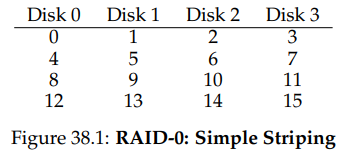
\includegraphics[width=\linewidth]{imgs/raid0_strip1}
\end{minipage}
\begin{minipage}{.55\linewidth}
  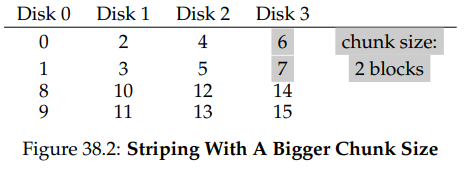
\includegraphics[width=\linewidth]{imgs/raid0_strip2}
\end{minipage}
\begin{itemize}
\item \textbf{stripe}: blocks in the same row (e.g. blocks 0, 1, 2, 3)
\item left:  1 block on each disk; chunk size: 4KB, stripe has $4\times 4 = 16$KB
\item right: 2 blocks on each disk; chunk size: 8KB, stripe has $4\times 8= 32$KB
\item small chunk size:
  \begin{enumerate*}[label={\alph*.},font={\color{lbl}\bfseries}]
  \item many files will get striped across many disks $\to \uparrow$ the parallelism of reads and writes to a single file
  \item the positioning time to access blocks across multiple disks $\uparrow \because$ the positioning time for the entire request is determined by the maximum
of the positioning times of the requests across all drives
  \end{enumerate*}
\item big chunk size:
  \begin{enumerate*}[label={\alph*.},font={\color{lbl}\bfseries}]
  \item reduces such intra-file parallelism; relies on multiple concurrent requests to achieve high throughput
  \item the positioning time to access blocks across multiple disks $\uparrow \because$ s reduce positioning time: single file on a disk, just the positioning time of that single disk
  \end{enumerate*}
\end{itemize}
\section*{Evaluating RAID Performance: 2 metrics + 2 workloads}
\begin{enumerate}
\item single-request latency: shows parallelism potential during one I/O op
\item stead-state throughput:
  \begin{enumerate*}[label={\alph*.},font={\color{lbl}\bfseries}]
  \item total bandwidth during concurrent requests
  \item critical in high-performance settings
  \item main focus of analysis
  \end{enumerate*}
\end{enumerate}
\begin{enumerate}
\item sequential:
  \begin{enumerate*}[label={\alph*.},font={\color{lbl}\bfseries}]
  \item requests come in large contiguous chunks: 1MB of data from block $x$ to $x+1$ MB
  \item common in many envs (e.g. file searching) and important for performance analysis
  \end{enumerate*}
\item random:
  \begin{enumerate*}[label={\alph*.},font={\color{lbl}\bfseries}]
  \item small individual requests
  \item each targets random disk locations: 4KB at addr 10, then 50,000, etc; important for DBMS
  \end{enumerate*}
\end{enumerate}
\begin{itemize}
\item sequential access: most efficient $\because$ minimal $T_{\text{seek}}$ and $T_{\text{rot.}}$ but maximum $T_{\text{dtransfer}}$. assume transfer rate: $S$MB/s
\item random access: least efficient $\because$ large $T_{\text{seek}}$ and $T_{\text{rot.}}$ but minimal $T_{\text{dtransfer}}$. assume transfer rate: $R$MB/s; generally: $S \gg R$
\item assume on average: a sequential transfers 10MB: a random trans: 10KB
\item on average seek time $T_{\text{seek}} = 7$ms, rotational delay $T_{\text{rot.}} = 3$ms, transfer rate of disk: 50MB/s
\item $S \approx 50$MB/s (bandwidth) $\because$ large time spent transferring; $S/R \approx 50$
\end{itemize}
\[
  S = \frac{\text{amount of data}}{\text{time to access}} = \frac{10\;\text{MB}}{T_{\text{seek}}+T_{\text{rot.}}+\frac{10\;\text{MB}}{50\;\text{MB/s}}} = \frac{10\;\text{MB}}{210\;\text{ms}} = 47.62\text{MB/s}
\]
\[
  R = \frac{\text{amount of data}}{\text{time to access}} = \frac{10\;\text{KB}}{T_{\text{seek}}+T_{\text{rot.}}+\frac{10\;\text{KB}}{50\;\text{MB/s}}} = \frac{10\;\text{KB}}{10.195\;\text{ms}} = 0.981\text{MB/s}
\]
\section*{RAID-0 Analysis (assume 4KB chunk size)}
\begin{itemize}
\item capacity: $N$ disks each with $B$ blocks, $N\cdot B$ useful capacity
\item reliability: perfect striping but any disk failure leads to data loss
\item performance: excellent, all disks utilized often in parallel
\item latency: good, identical to that of a single disk
\item stead-state throughput: sequential = $N \cdot S$MB/s; random = $N\cdot R$MB/s
\end{itemize}
\section*{RAIDs simplified summary}
\begin{itemize}
\item Mirrored Systems Write Performance:
  \begin{itemize}
  \item Average seek time is higher than single disk
  \item Uses maximum of two seeks (one per disk)
  \item Random write performance slightly lower than single disk
  \end{itemize}
\item RAID-4/5 Parity Updates
  \begin{itemize}
  \item First read of old parity: requires full seek and rotation
  \item Second write of parity: only needs rotation
  \item RAID5 has replaced RAID4 in most marketplace because RAID-5 is basically identical to RAID-4 except in the few cases where it is better. The only place where RAID4 is still in use is systems that know they will never perform anything other than a large write, thus avoiding the smallwrite problem altogether; in those cases, RAID-4 is sometimes used as it is slightly simpler to build.
  \end{itemize}
\item Mirrored RAIDs have 2× perf. penalty compared to other approaches
\item RAID 01: two stripes (RAID0) that are mirrored (RAID1)
\item RAID 10: stripe (RAID0) a set of mirrored devices (RAID1)
\end{itemize}
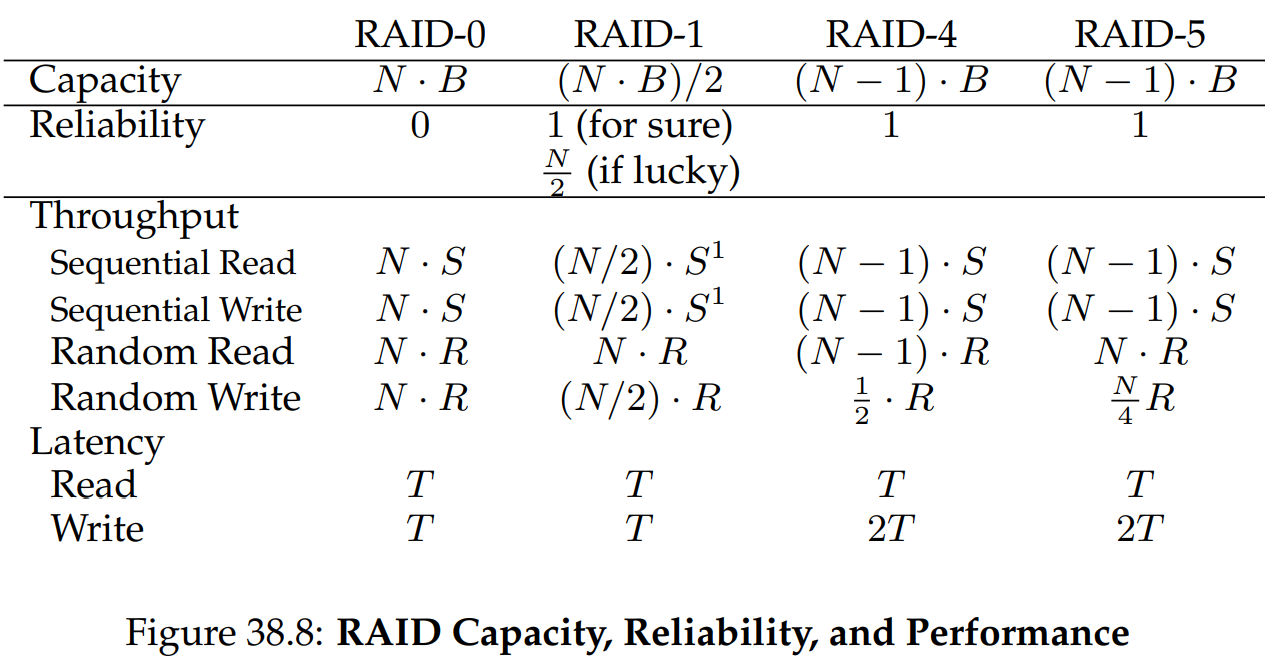
\includegraphics[width=\linewidth]{imgs/raid_compare}
\begin{minipage}{.5\linewidth}
  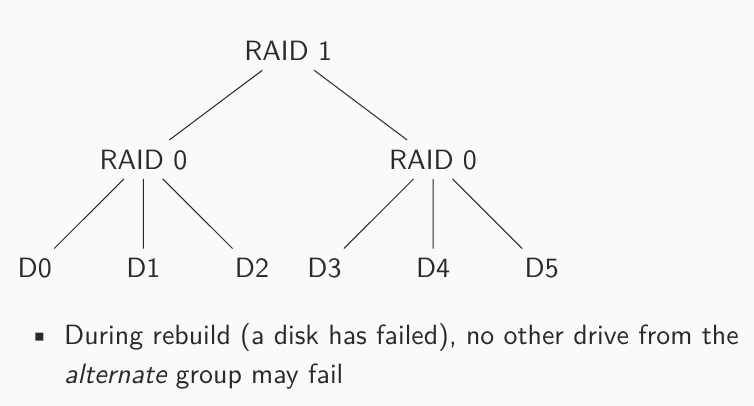
\includegraphics[width=\linewidth]{imgs/raid01}
\end{minipage}
\begin{minipage}{.5\linewidth}
  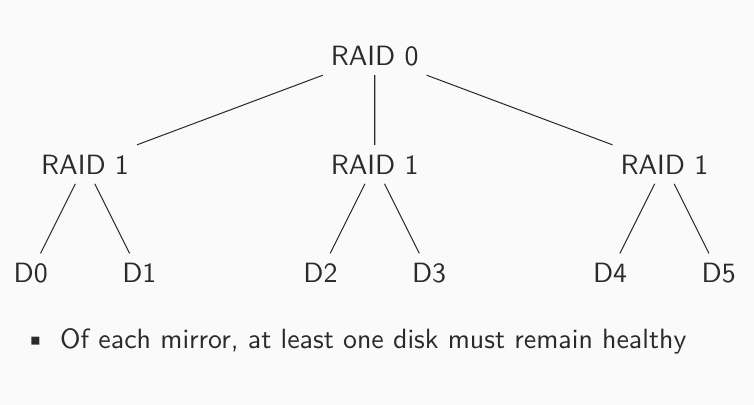
\includegraphics[width=\linewidth]{imgs/raid10}
\end{minipage}
%%%%%%%%%%%%%%%%%%%%%%%%%%%% FILE SYSTEM %%%%%%%%%%%%%%%%%%%%%%%%%%%%
\section*{FFS writes a lot to create a new file of size one block}
\begin{itemize}
\item one for a new inode, one to update the inode bitmap
\item one to the directory data block that the file is in
\item one to the directory inode to update it
\item one to the new data block that is a part of the new file
\item one to the data bitmap to mark the data block as allocated
\end{itemize}
Although FFS places all of these blocks within the same block group, FFS incurs many short seeks and subsequent rotational delays and thus performance falls far short of peak sequential bandwidth
\section*{Reading a file from disk using LFS}
Assume we have nothing in memory to begin. The first on-disk data structure we must read is the checkpoint region. The checkpoint region contains pointers (i.e., disk addresses) to the entire inode map, and thus LFS then reads in the entire inode map and caches it in memory. After this point, when given an inode number of a file, LFS simply looks up the inode-number to inode-diskaddress mapping in the imap, and reads in the most recent version of the inode. To read a block from the file, at this point, LFS proceeds exactly as a typical UNIX file system, by using direct pointers or indirect pointers or doubly-indirect pointers as need be. In the common case, LFS should perform the same number of I/Os as a typical file system when reading a file from disk; the entire imap is cached and thus the extra work LFS does during a read is to look up the inode’s address in the imap.
